\section{Технический проект}
\subsection{Общая характеристика организации решения задачи}

Поставлена цель разработать программу, работающую на спецификации OpenGL, способную загрузить массив трёхмерных данных и графически осуществить их визуализацию на экране для пользователя.

Трёхмерный графический движок на высоком уровне представляет из себя структуру основных классов - примитивов для построения основной минимальной трёхмерной графики: массив координат точек, массив нумерации граней, матрица проекциий, объект виртуальной камеры, набор текстур и программ шейдеров, которые все вместе осуществляют отрисовку объекта на трёхмерной сцене.

На более низком уровне трёхмерный движок представляет из себя набор комманд и программ для работы с видеоадаптерами и буфферами памяти системы. Из данного набора команд и программ была создана основа разрабатываемой программы, работающей под спецификацией OpenGL.

В движке используется разработанная программа парсера. Парсер считывает структуру файлов трёхмерных объектов. Массив трёхмерных данных считывается последовательно и обрабатываются синтаксическим анализатором. На основе данных считанных объектов формируются массивы координат вершин, индексов и координат текстур.
\subsection{Обоснование выбора технологии проектирования}

Обоснованием выбора технологии проектирования послужило задание на разработку, целью которой являлось создание программы, работающей на спецификации OpenGL. Соответственно, была выбрана последняя выпущенная версия OpenGL 4.6. А выбором среды и языка проектирования интерфейса и создания программы послужило удобство и простота использования языка C\# в среде Visual Studio.

\subsection{Описание используемых технологий и языков программирования}

В процессе разработки программного обеспечения было использовано программное средство IDE Visual Studio, а также использованы языки программирования C\# - при создании интерфейса программы и C - при работе со спецификацией OpenGL.

\subsubsection{Язык программирования C\#}

\paragraph{Достоинства языка C\#}

C\# - многоцелевой объектно-ориентированный язык программирования. Относится к семье с С-подобным синтаксисом, наиболее идентичен C++ и Java. Имеет более расширенный спект функций, чем у предшественника - C++, чем является намного проще в использовании, но также из-за своих удобств является более высокоуровневым, что делает его ориентированным в основном на разработку десктопных приложений.

\paragraph{Недостатки языка C\#}

Язык C\# является немного более высокоуровневым, чем C++, поэтому менее тесно взаимодействует с аппаратной частью вычислительных систем, что сильно  ограничивает его функционал в случаях разработки низкоуровневых приложений, где работа с памятью системы и прямое взаимодействие с аппаратной частью необходимо.

\subsubsection{Спецификация OpenGL 4.6}

OpenGL ориентирован на две задачи:
\begin{itemize}
	\item Скрыть сложности адаптации различных 3D-ускорителей, предоставляя разработчику единый API;
	\item Скрыть различия в возможностях аппаратных платформ, требуя реализации недостающей функциональности с помощью программной эмуляции.
\end{itemize}

\paragraph{Достоинства спецификации OpenGL}

Главным достоинством OpenGL является его гибкость, открытый код и низкие требования к ресурсам устройства.

\begin{itemize}
	\item Возможности данной спецификации позволяют разработчику создавать полностью уникальные и подстроенные под особую специфику задач приложения;
	\item устройство данной графической библиотеки позволяет запускать и поддерживать приложения с максимально возможной производительностью;
	\item это низкоуровная библиотека, которая позволяет напрямую работать с аппаратным железом - управлять памятью системы и буффером видеоадаптера;
	\item самодостаточность спецификации даёт возможность не использовать дополнительные плагины и библиотеки в реализации визуализации графики;
	\item полная мультиплатформенность - OpenGL работает на всех платформах, языках и устройствах.
\end{itemize}

\paragraph{Недостатки спецификации OpenGL}

\begin{itemize}
	\item Низкоуровневость библиотеки - для неопытного, или же начинающего разработчика это может стать главной проблемой в работе с OpenGL, потому как для создания программного обеспечения, использующего спецификацию OpenGL, необходимы глубокие знания об основах трёхмерной графики и линейной алгебры, а также иметь минимальное представление об обмене данными в видеоадаптерах на аппаратном уровне;
	\item данная технология в настоящее время считается уже устаревшей, и была заменена более современным API Vulcan;
	\item с выходом новых видеокарт, их спектр возможностей, как и реализуемых функций расширился, так что новые функции, такие как DLSS и RTX не вошли в стандарт спецификации OpenGL.
\end{itemize}

\subsection{Диаграмма классов и компоненты программы}

Диаграмма классов описывает виды классов программы и различного рода связи, которые существуют между элементами. На диаграммах изображаются также атрибуты классов, их функции, принимаемые значения, а также ограничения описывающие взаимодействие между классами. Вид и представление диаграммы классов напрямую зависит от уровня абстракции: классы могут быть показаны в качестве сущностей предметной области или же как элементы частей программного обеспечения. В нашем случае, на рисунке \ref{diagram3:image} показана диаграмма классов, которые являются элементами программной среды. 

Атрибуты в диаграмме описывают свойства объектов класса. Элементы класса обладают своей индивидуальностью из-за различий в их параметрах, а также связях с другими объектами. 

В большинстве случаев, в данном программном обеспечении большинство классов существуют в единственном экземпляре, из-за их уникальной сущности. Как пример, можно привести класс, определяющий виртуальную камеру, которая должна существовать в единственном экземпляре, ведь на один экран должно выводиться одновременно лишь одно изображение.

Но несмотря на это, структура классов в данном программном обеспечении всё равно является объектно ориентированной, благодаря чему внутри неё был реализован механизм управления объектными моделями, текстурами и другими элементами, которые все связаны между собой наследуемостью классов, а также существует возможность дальнейшего развития и расширения общей системы классов, путём добавлением в неё новых элементов.

\begin{figure}[H]
\center{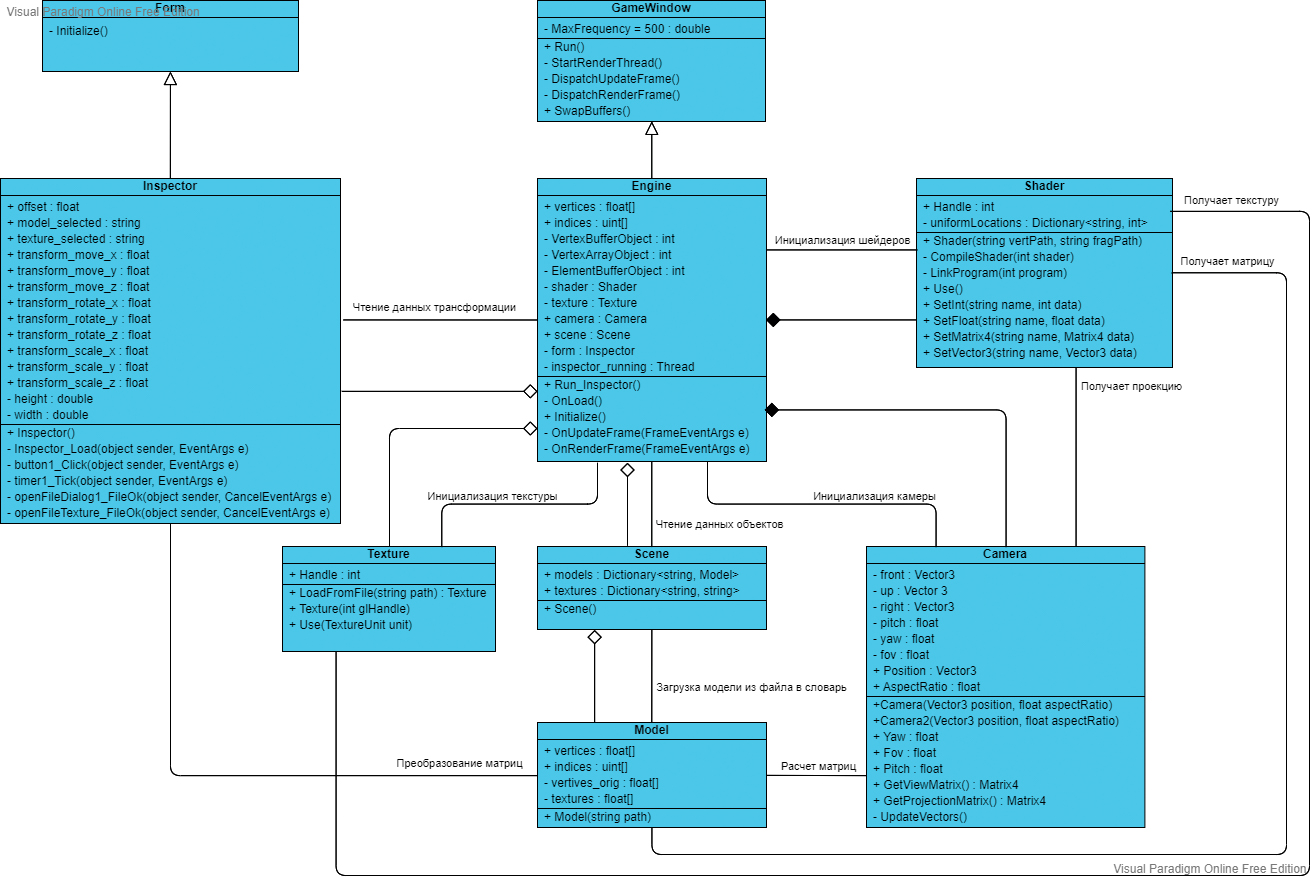
\includegraphics[width=1\linewidth]{diagram3}}
\caption{Диаграмма классов программы}
\label{diagram3:image}
\end{figure}

Все элементы программы имеют общий родительский элемент в виде главного класса - обработчика событий, который является главным элементом и центром всей программы.

\begin{itemize}
	\item Класс Model является каркасом трёхмерной модели. Выполняет роль приёма, хранения и передачи массива трёхмерных данных для обработчика триангулярных примитивов. При создании выполняет чтение и преобразование в массивы вершин и индексов, загруженного файла с данными трёхмерного объекта;
	\item класс Texture при инициализации выделяет место в буффере памяти видеоадаптера для загруженной в программу текстуры, а также обрабатывает настройки параметров её отображения;
	\item класс Scene выполняет роль хранилища моделей и изображений, а также выступает виртуальной сценой, на которой находятся все трёхмерные объекты и остальные элементы, учавствующие в визуализации. При инициализации выполняет загрузку данных массивов моделей и привязанных к ним файлов текстур, которые уже были раннее загружены в проект;
	\item класс Shader является программой настройки конечной визуализации, и при инициализации создаёт подпрограмму в общей графике, для преобразования растеризированного изображения внутри буффера памяти видеоадаптера, для отображения текстур и освещения;
	\item класс Camera является матрицей преобразования, для корректного отображения перспективы виртуального трёхмерного вида сцены, и для того, чтобы конечный вид проекции сцены был перспективным, а не ортографическим;
	\item класс Engine является основой проекта, графическим движком, который инициализирует всю графику, принимает события ввода пользователя, отвечает за обновление кадров и управление всеми настройками, а также связывает все классы между собой;
	\item класс Inspector является частью пользовательского интерфейса, и представляет из себя окно взаимодействия между пользователем и программой. Служит для того, чтобы пользователь осуществлял загрузку собственных массивов трёхмерных данных моделей и текстур в проект, а также осуществлял указанные аффинные преобразования над загруженными моделями.
\end{itemize}

Также отдельно стоит указать класс GameWindow - это родительский класс для класса Engine. По своей сути он является измененным элементом класса Form от WindowsForms и не принимает прямого участия в работе проекта, но содержит формальные данные, необходимые для корректной инициализации главного окна проекта.

\subsection{Описание работы парсера}

В результате тесной работы со множеством различных файлов трёхмерных данных с расширением *.obj, возникла необходимость автоматизировать загрузку и интерпретацию этих данных для программы. Для решения данной задачи был разработан специальный алгоритм программы парсера.

Парсер, или же синтаксический анализатор - часть программы, которая преобразовывает текстовые входные данные в структурированный формат.

Главный принцип работы разрабатываемого приложения завязан на использовании файлов трёхмерных данных формата *.obj. Это формат файлов описания геометрии, разработанный в Wavefront Technologies. Он содержит только 3D геометрию, а именно: позицию каждой вершины, связь координат текстуры с вершиной, направления нормалей, а также параметры, которые создают триангулярные примитивы. Исходя из этого, необходимо, чтобы парсер мог разделить все эти данные на отдельные массивы, которые будут использовать программа. В заключение вышесказанного, можно построить схему, по которой должен будет работать парсер, как показано на рис.~\ref{diagram4:image}, где изображён общий принцип работы подпрограммы парсера.

\begin{figure}[ht]
	\center{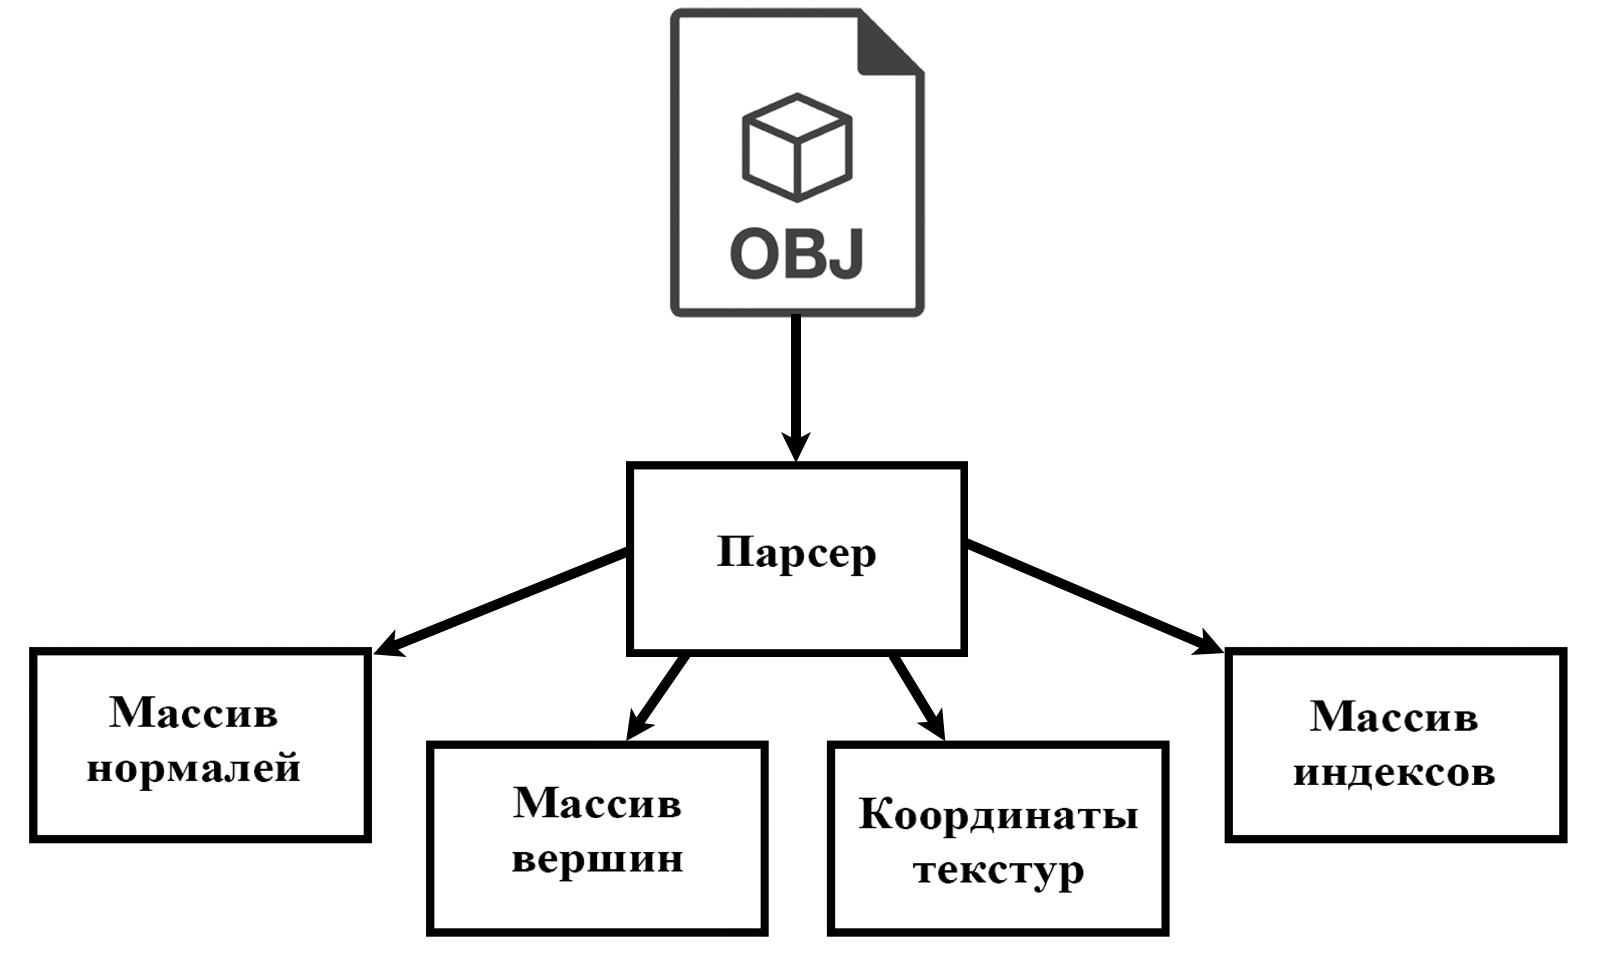
\includegraphics[width=1\linewidth]{diagram4}}
	\caption{Принцип работы программы парсера}
	\label{diagram4:image}
\end{figure}

Так как парсер - это не отдельный класс, то его подпрограмма будет находиться в классе Model, чтобы в будущем каждый элемент этого класса мог сразу автоматически интерпретировать и структурировать данные своей модели в массивы трёхмерных данных. Таким образом, несмотря на хранение в программе трёхмерных данных в файлах формата OBJ, они сразу бы могли структурироваться под стандарты программы, при инициализации элементов класса Model с указанием нужного файла.


\subsection{Проектирование пользовательского интерфейса}

Графический прототип интерфейса, показанный на рис.~\ref{maket2:image} демонстрирует, какие элементы пользовательского интерфейса будут включены в конечную реализацию программы.

\begin{figure}[H]
\center{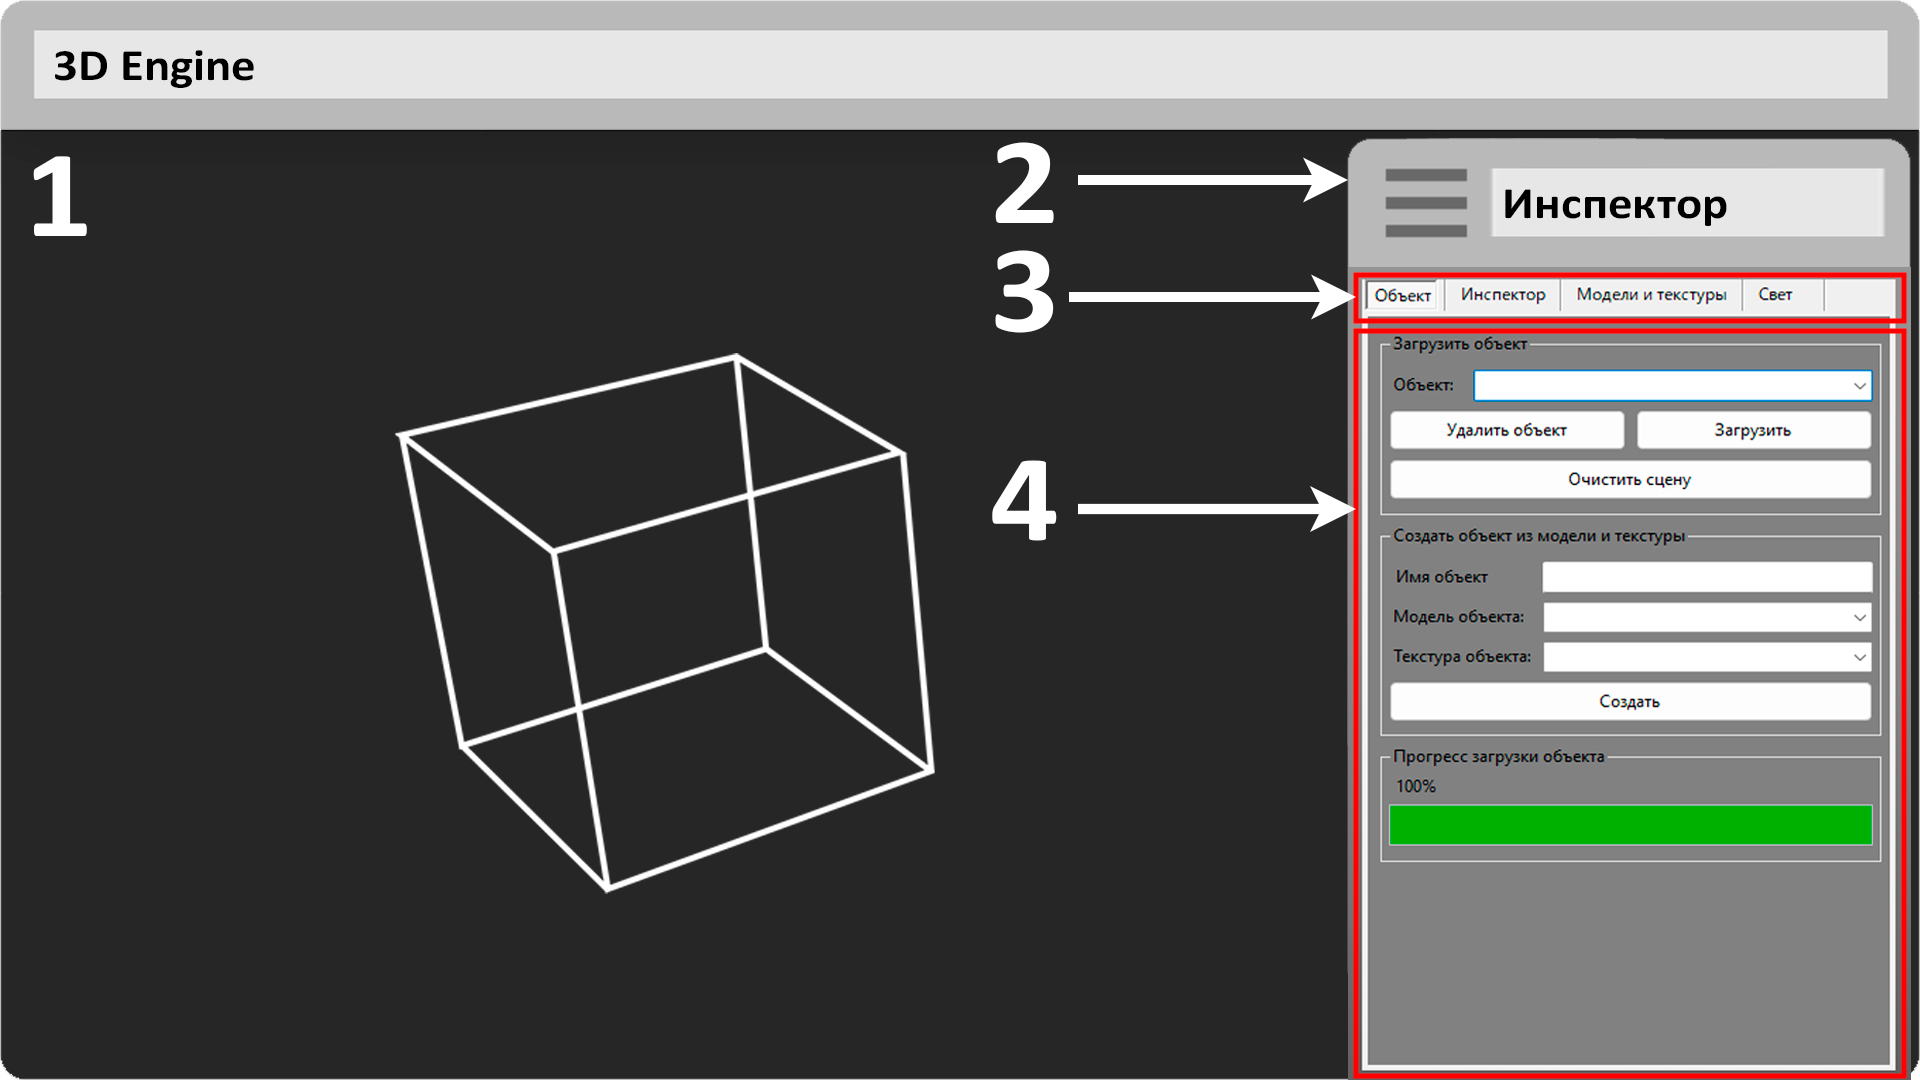
\includegraphics[width=1\linewidth]{maket2}}
\caption{Прототип пользовательского интерфейса}
\label{maket2:image}
\end{figure}

Описание элементов интерфейса, показанного на рис.~\ref{maket2:image}:
\begin{enumerate}
	\item Главное окно программы. Выводит визуализированные данные на экран.
	\item Окно инспектора.
	\item Вкладки окон инспектора.
	\item Активное меню вкладки инспектора.
\end{enumerate}

\subsubsection{Главное окно программы}

Главное окно программы представляет из себя виртуальную трёхмерную среду с одноцветным фоном. Оно служит для отображения визуализации трёхмерных моделей, которые пользователь загрузит в программу. Также данное окно является частью пользовательского интерфейса с интуитивной функцией ввода - пользователь может управлять направлением перспективы взгляда камеры, зажав правую кнопку мыши и направляя курсор в нужную сторону, чтобы управлять камерой и осматриваться в виртуальном пространстве. А используя колесо прокрутки, пользователь может отдалять и приближать угол обзора.

Управление перемещением камеры в пространстве также осуществляется в главном окне программы, с помощью клавиатуры:
\begin{itemize}
	\item клавиша «W» – переместить камеру вперёд по направлению взгляда;
	\item клавиша «A» – переместить камеру вправо относительно направления взгляда;
	\item клавиша «S» – переместить камеру назад по направлению взгляда;
	\item клавиша «D» – переместить камеру влево относительно направления взгляда;
	\item клавиша «левый Shift» – поднять камеру вверх, по координате +Y;
	\item клавиша «левый Ctrl» – опустить камеру вниз, по координате -Y;
\end{itemize}

\subsubsection{Окно инспектора}

Инспектор - это дополнительное окно, расположенное по краю справа, поверх главного окна. Оно служит вспомогательным элементом интерфейса, чтобы пользователь мог взаимодействовать и управлять элементами внутри виртуальной сцены. Например, выполнять преобразование массива данных трёхмерной модели - перемещать её в пространстве, наклонять под определённым углом и прозводить растяжение или сжатие, и всё это по всем трём координатам.

\subsubsection{Вкладки окон инспектора}

Меню со вкладками окон инспектора, где пользователь может выбрать одну трёх вкладок, чтобы переключать и менять содержание активного меню инспектора.

\subsubsection{Активное меню вкладки инспектора}

Показывает основной интерфейс меню инспектора. Инспектор имеет три разных активных меню, и содержание окна инспектора будет меняться, в зависимости от выбранной вкладки:
\begin{itemize}
	\item Вкладка "<Объект"> - в данной вкладке пользователь может выбрать из выпадающего списка модели и текстуры, которые он хочет загрузить и визуализировать на виртуальной сцене. Также данная вкладка имеет ещё два раздела: раздел трансформации, в котором пользователь может задать значения для преобразования данных на сцене и раздел консоли, в которую будут выводиться данные о выполненных операциях, и информация об ошибках, если в программе произойдут сбои.
	\item Вкладка "<Инспектор"> - это информационная вкладка, в которой показаны точные координаты и наклон камеры, а также данные о произведенных преобразованиях над моделью: смещении, наклона и масштабировании.
	\item  В последней вкладке "<Модели и текстуры"> содержится весь список доступных моделей и текстур в программе, загруженных пользователем. Также в ней пользователь может осуществлять непосредственно саму загрузку массивов трёхмерных данных с расширением *.obj в программу и изображений текстур с расширением *.png и *.jpg.
\end{itemize}